% Chapter sectioning]
%\protect\hypertarget{_Toc53412554}{}{}
\section{Scripting tutorial}

If you are completely new to scripting and programming in general, the thought of using TES script might be a little daunting -- I have therefore written an extended tutorial that will walk you through making your first script. I will also explain the main elements of the scripting language as we go. There will be other explanations on the way, but the key instructions will be in \textbf{bold} print.

\hypertarget{lets-get-going}{%
\subsection{Let's get going!}\label{lets-get-going}}

We start by opening the script editor: \textbf{Start up the TES Construction Set, open the Morrowind.esm file and then select Edit Scripts from the Gameplay menu to open the scripting window.}

\hypertarget{the-scripting-window}{%
\subsection{The scripting window}\label{the-scripting-window}}

You enter the script editor either by \textbf{selecting Gameplay -- Edit Scripts from the menu}, by clicking the edit script button (the pencil) in the taskbar or by accessing it from an Object or NPC dialogue, by clicking the button with the ellipses {[}\ldots{]} next to the script field. The editor window is pretty basic:

% Graphic here is on another page because the margins are different than the .doc

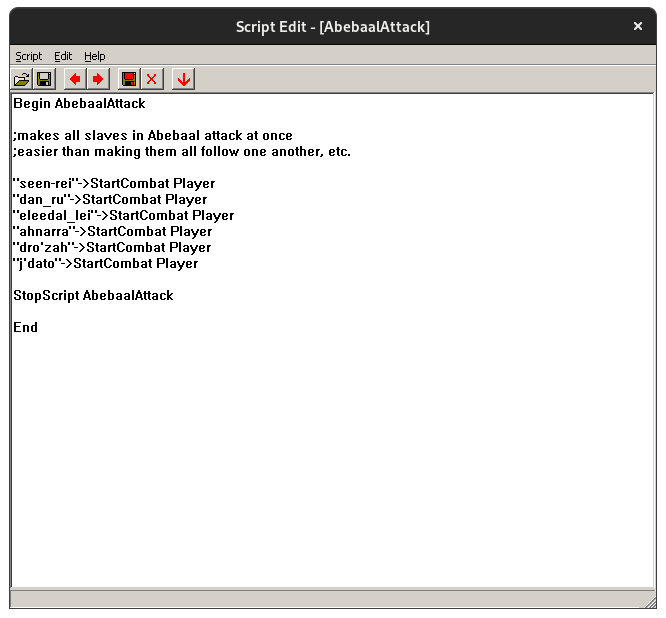
\includegraphics{media/script-abebaal-attack.png}

Let's have a look at the buttons in the taskbar, from left to right: \emph{Open} lets you select a script to edit. \emph{Save} error checks the current script and compiles it or gives out error messages -- note, however, that the plugin and thus the script is not really saved to disk at this time. When programming large scripts frequently use the save command in the main TESCS window after you have saved the script here, just in case the TESCS crashes.

Note that if you edit the script and suddenly hit "save plugin" to backup in the middle of the work, your updated script will NOT be saved with it. You must save it manually first. Also, if you just close script window, it doesn't mean that script will be saved. You must take care of it yourself (Thanks to Kir for this tip).

\emph{Forward and Backward arrows} jump to the next or previous script, respectively (alphabetical order). If you give your scripts a common tag, that will make it easier to jump between the different scripts of your project, e.g. start every script name with AA\_Scriptname this will put them right at the beginning of the list and keep them neatly together. \emph{Compile all} recompiles all scripts (what's this good for? I don't really know). Finally, the \emph{delete} button deletes a script and the last "\emph{arrow down}" button closes the script window.

The help menu gives quick access to the function and command pages of the helpfile (of moderate utility, hence the creation of this manual!)

You can cut, copy, and paste from and into the editor window by using the Windows standards ctrl-c for copy, ctrl-x for cut and ctrl-v for paste.

\hypertarget{what-do-we-want}{%
\subsection{What do we want?}\label{what-do-we-want}}

Before we really start writing our tutorial script we should decide what we want it to do. For this tutorial I decided we are going to make a \textbf{Riddle Chest: The chest will ask a riddle and only the right answer will open the chest. If the player provides the wrong answer, a trap will go off, hurting the player, and the chest can't be opened.}

That's a fairly complex undertaking, but we will take it step by step.

\hypertarget{writing-a-script}{%
\subsection{Writing a script}\label{writing-a-script}}

Ok, once you've got the Edit Script window open, \textbf{click into the main part of the window.} That is where you will write your script.

\hypertarget{naming-a-script-begin-and-end}{%
\subsubsection{Naming a script: Begin and End}\label{naming-a-script-begin-and-end}}

First of all we must give our script a name -- every script must start with the declaration of this name. \textbf{So please type:}

\begin{lstlisting}
Begin my_first_script
\end{lstlisting}

\textbf{into the editor window}. Note the underscores: Your name should be one word. Also note that the script language is not case sensitive, so \emph{Begin} could also be written without the capital letter: \emph{begin}. This name is the handle by which the script will be known in the TESCS. Try hitting the save button now: you will get an error message about "you need to end your script with end scriptname. So, for the editor to recognize the script we also need to indicate an
end: \textbf{next, write}

\begin{lstlisting}
End
\end{lstlisting}

\textbf{in a new line below the above}. As you see we can omit putting the name of the script in this line again, just \emph{end} will do. When you hit \emph{safe} now, you will see the name appear in the title bar of the script editor, indicating that the script has been accepted. This is the shortest script possible - and of course it doesn't do anything at all.

\hypertarget{detecting-an-action-by-the-player}{%
\subsubsection{Detecting an action by the player}\label{detecting-an-action-by-the-player}}

Next, we need a way to determine whether the player tries to open the chest. In TES Script we distinguish between Objects, Functions and Commands --

\textbf{Objects} are all the things in the game world, be they visible objects, creatures, NPCs or just sounds.

\textbf{Functions} are the all the "words" of TES Script that let us either manipulate these objects or let us gather information about them.

\textbf{Commands} are those "words" that structure the scripting language, but do not operate on any Game objects -- an example is the word "Begin" we used to tell the script editor about the name of our script.

To tell the game which object it is supposed to perform a given function on we can use the "arrow", or "fix" : -\textgreater{} (really just a hyphen and a greater-than sign). You specify the object for the function on the left (we also call this the calling object) and the function to be performed on the right:

Object\_ID-\textgreater function, {[}parameters{]}

A function may or may not have parameters. Parameters could be other object ID's, numbers and in some cases, variables.

What we need for our riddle chest is the OnActivate function: this is an informative function that tells us whether the player has "activated" an object in the game world or not. This function returns a value of 1 (which means "true" in programming terms) if the object has been activated, that means the player targets it and presses the "use" button (space, by default). So what we need to do is check if OnActivate becomes "true" anytime in the game. \textbf{So edit your script to look like this:}

\lstinputlisting{scripts/my_first_script01.txt}

A couple more things need to be explained here: The "\emph{if}" command is there to check a condition -- whenever the expression in the parentheses is "true" the following lines of code will be executed until the "endif" command is encountered. The "==" checks if an expression (in our case the "OnActivate" function) on the left of it is equal to the expression on the right of it (in our case to 1). If you forget the \emph{endif} command after an if command, the editor will complain with an error message. The ";" semicolon denotes a comment -- whatever you write behind the semicolon will be ignored when the script is run. If you ever write larger scripts you should learn to love this possibility.

\hypertarget{writing-text-and-obtaining-decisions-from-the-player}{%
\subsubsection{Writing text and obtaining decisions from the player}\label{writing-text-and-obtaining-decisions-from-the-player}}

Now we want our trapped chest to ask the player a riddle. For this we use the MessageBox function that allows us to display some text on the screen and also to display choices that the player can select from. Unfortunately Morrowind has no option to have the player type in the answer to our riddle, so we will have to give multiple choices. The line for that could read:

\begin{lstlisting}
MessageBox "Voiceless it cries, wingless flutters, toothless bites,
mouthless mutters. What is it?", "Bat", "Old woman", "Wind", "Wraith"
\end{lstlisting}

The first text is the text actually displayed in the box, the other texts, separated by commas tell the game to make "buttons", with the text given displayed.

But how do we ensure that the riddle is asked only the first time we try to open the chest and not every time? We now come to a very central point: the use of do-once conditions and state variables. Most of the problems that beginners encounter with scripting for Morrowind have their roots in misunderstanding how the scripts are actually executed and how scripts should accordingly be structured. So let's have a look at this.

\hypertarget{how-local-scripts-are-executed}{%
\subsubsection{How local scripts are
executed}\label{how-local-scripts-are-executed}}

Every script that is attached to an Object or an NPC (local script) is executed \emph{every frame the game displays on screen} while the cell with the object is active (indoors only the cell the NPC is currently in is active, outdoors the PC's cell and all adjacent cells are active). So the \emph{complete script} (not just one line of it) is executed 10-60 times a second or however fast your computer runs the game! It is best to imagine every local script wrapped in a big ``while-loop'':

\begin{lstlisting}
while (Object is in active Cell)

{[}Your script code{]}

endwhile
\end{lstlisting}

This is the reason why the following script spits out a continuous stream of messages (if attached to an Object or NPC in the same cell as the player). Try it, if you want:

\lstinputlisting{scripts/Message_script.txt}

This example is relatively harmless, but imagine what happens if you would use a line of code that adds an item to the players inventory, or places a monster next to him, etc.!

For this reason, ``Do Once'' constructions are very essential and something you will probably use a lot while scripting for Morrowind. So, let's go on with our tutorial script: we need to declare a variable and use it to make sure the message is only displayed once. \textbf{Change the script to the following:}

\lstinputlisting{scripts/my_first_script02.txt}

(Please note that the MessageBox command should be in one line in the editor!)

"\emph{Short controlvar}" declares a new variable I called "\emph{controlvar}", of type short. For the moment it's enough to know that this is variable that will contain integers (whole positive or negative numbers). A variable is a "placeholder" that can take on different values. The \emph{if} command we already know, the \emph{set} command is new, but simple enough -- it sets our variable that had the value 0 before (all variables start out at zero when declared) to 1. This, in connection with the \emph{if ( controlvar == 0 )} command provides a do-once condition -- the next frame the script is executed after the variable was set to 1 the if condition will be false and the message box will not be displayed again.

Now our script is already capable of being run, so lets test it:

\begin{itemize}
\item
  \textbf{Save the script and close the script editor window.}
\item
  \textbf{Go to the TES construction set, Object window, select the
  container tab and open "chest\_small\_01".}
\item
  \textbf{Change the ID of the chest to "tutorial\_chest"}
\item
  \textbf{In the script dropdown field, select my\_first\_script}
\item
  \textbf{Save the object as a new object, save the mod, and quit the
  construction set. Start Morrowind and load a savegame.}
\item
  \textbf{Now bring down the console (usually the \textasciitilde{} key,
  or whatever you have to the left of the "1" on the main keyboard) and
  in the console window, type:}\\
  PlaceAtPC tutorial\_chest 1,1,1\\
  \textbf{and hit return.}
\end{itemize}

Take a step back (err, let your player character step back, that is!); you should now have a little chest sitting on the floor right in front of you. Clicking on it should bring up our message, which should look like this:

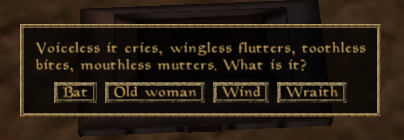
\includegraphics{media/image3.png}

Clicking on those buttons will just close the messagebox for the moment, and clicking on the chest again, nothing should happen either -- which is good, it means our do-once condition works.

\textbf{Ok, leave Morrowind and go back to the editor, and load your plugin again.}

We now need to figure out which answer the player selects, and script appropriate reactions for right and wrong answers. The function to test the selected answer is "GetButtonPressed". This function returns a number depending on which of the buttons of a message box has been clicked on with the mouse. It will return "0" for the first button ("bat" in our example) and 1, 2, 3 etc. for the following buttons, in the order you listed them in the messagebox function. While no answer
has been selected, the function will return --1, so we have to take care of that, too.

The "Activate" function will make our chest open, in fact activate will simply trigger the standard action that would usually be performed when you "use" the selected object -- e.g. doors would swing open, NPCs would initiate dialogue etc.

The following update to our script also demonstrates how you can use a control variable to force MW to process functions one after the other, although the complete script is processed every frame of the game: simply increment the control variable and test it in a series of if -- elseif statements. This is a very safe way of scripting for MW -- it may not always be necessary, but it's safe.

Please edit the script to the following:

\lstinputlisting{scripts/my_first_script03.txt}

Take a look at the part that starts with "\emph{if (controlvar == 1)}". We have set controlvar to 1 as soon as the chest got activated. Now we test for which button is being pressed. We do this by assigning the new variable "\emph{button}" a value returned by \emph{GetButtonPressed}. Since the script is still running, even while the game seemingly pauses to await your decision, we first test if no button has been selected yet -- return tells the game engine to stop processing the script for this frame.

Our correct answer was "wind" which corresponds to button number two -- if button number two gets pressed, we will tell the player that he gave the right answer, and "activate" will open the chests inventory in the usual way.

All other values of button mean that the player has selected a wrong answer, so we can use the "\emph{else}" command here. In this case we tell the player what a fool he was and the chest is not activated.

Now look at the little addition at the top of the script:

% Excerpt from external script. my_first_script03 [firstline=6, lastline=13]

\begin{lstlisting}
	If ( OnActivate == 1 )
	
	If ( controlvar == 0)
	
	MessageBox "Voiceless it cries, wingless flutters, toothless bites,
	mouthless mutters. What is it?", "Bat", "Old woman", "Wind", "Wraith"
	
	Set controlvar to 1
	
	elseif controlvar \textgreater{} 1
	
	activate
	
	endif
	
	endif
\end{lstlisting}

This means that, whenever the chest is activated in the future, it will only open if controlvar is greater than 1. Check above: when the player provides the wrong answer in the riddle, controlvar is set to --1, so he will never be able to open the chest. But if he knew the right answer, \emph{controlvar} is set to 2, and from now on the player can open the chest as often as he likes. Save and run your plugin, and test as described above.

\hypertarget{your-first-bug}{%
\subsubsection{Your first bug}\label{your-first-bug}}

Now, you will probably have noticed that the script does almost -- but not quite -- what we wanted. After clicking the correct answer, the chests inventory doesn't open as intended. Now, the logic above seemed fine, so what is wrong? \textbf{Let's try the following (change the corresponding part of your script according to the fragment below):}

% Excerpt from external script. [firstline=, lastline=]

\begin{lstlisting}
	if (controlvar == 1)
	
	set button to GetButtonPressed
	
	if ( button == -1 )
	
	return
	
	elseif ( button == 2 )
	
	MessageBox "The answer was correct"
	
	set controlvar to 2
	
	else
	
	MessageBox "The answer was wrong"
	
	set controlvar to -1
	
	endif
	
	elseif ( controlvar == 2 )
	
	Activate
	
	endif
\end{lstlisting}

See how I moved the activate command to the section that tests for controlvar == 2? This provides a cleaner sequence of events, and as I mentioned above, this can be very important when scripting for Morrowind -- always try to avoid doing too many things at once! \textbf{Well, run and test it.}

Great, now the inventory opens as we wanted, but what is this? The cursor is real slow, and we can't close the inventory! Look above -- \emph{controlvar} was set to two, and remains there, we do not change it again -- therefore the game now gets continuous "\emph{Activate}" commands each time the script is processed (every frame)! That's why we can't close the inventory -- it gets reopened immediately. \textbf{So change the following part of the script:}

% Excerpt from external script. [firstline=, lastline=]

\begin{lstlisting}
	elseif ( controlvar == 2 )
	
	Activate
	
	Set controlvar to 3
	
	endif
\end{lstlisting}

\textbf{Test again}: now everything works the way we wanted. I hope I have not confused you with the above excursion into the process of debugging, but it is a very important thing to know about -- you will constantly have to rethink your scripts and try different ways of doing it to be successful.

What is still missing? The trap effect of course!

\hypertarget{putting-a-spell-on-the-player}{%
\subsubsection{Putting a spell on the player}\label{putting-a-spell-on-the-player}}

Our chest will put a curse on the player if he fails to answer the riddle.

First go to the spellmaking tab in the editor, right click and select "new". Give the spell the ID "Frost\_Curse", name it "Frost Curse" and make it type "curse" then give it a magnitude of e.g. 1-5. It should look like in the picture below.

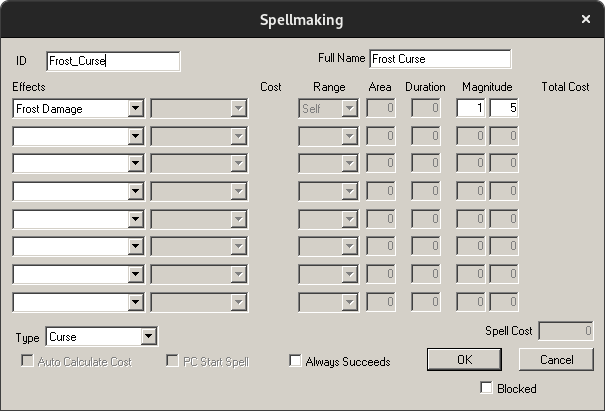
\includegraphics{media/frost-curse.png}

Now, we need to put this curse on the player. For this we use the \emph{AddSpell} function. After some time we will remove the curse again using the \emph{RemoveSpell} function, for this we need to make a timer. Edit your script again:

\lstinputlisting{scripts/my_first_script04.txt}

Let's go over this. Player-\textgreater AddSpell, "Frost\_Curse" puts the curse we created earlier on the player. Note how we need to use "Player-\textgreater" to make sure the effect really targets the player. Otherwise we would curse the chest (which is the default object, because the script is attached to it), which wouldn't make a lot of sense\ldots{}

% Excerpt from external script. [firstline=, lastline=]

This bit:

\begin{lstlisting}
	Float timer
	
	Set timer to ( timer + GetSecondsPassed )
	
	if timer \textgreater{} 10
\end{lstlisting}

\ldots that is how you make a timer in Morrowind. \emph{GetSecondsPassed} is a function that returns the time in seconds that has passed since the last frame. Since this is usually a fraction of a second (as the script gets called every frame), it is only natural that we need a float variable for this purpose -- a variable that can store numbers with decimals. So when the timer has been running for 10 seconds we remove the curse again, and make sure we do this only once:

% Excerpt from external script. [firstline=, lastline=]

\begin{lstlisting}
	Player-\textgreater RemoveSpell, "Frost\_Curse"
	
	set controlvar to -2
\end{lstlisting}

Ok, save and test your mod. Works fine now, doesn't it? Well, almost. Try the following: let yourself be cursed, and then open your inventory. Wait. See how the curse terminates after some time, without hurting you? Of course: the script is still running, but spell effects are only calculated while in game, not while you are in the menu. We don't want the player to get off the hook so easily, so we need to put something in our script that stops it from processing when we are in menu mode. Luckily there is the \emph{MenuMode} function, which returns 1 when you enter the menu. So we can put this at the start of our script:

% Excerpt from external script. [firstline=, lastline=]

\begin{lstlisting}
	If ( MenuMode == 1 )
	
	Return
	
	Endif
\end{lstlisting}

Remember, return tells the game to stop processing the script for this frame.

Ok, now we have our final working script. Congratulations! If you want, experiment a little more with this script: Put the chest into a location in the game and lock it. Then try unlocking it (Unlock function) with the script in addition to activating it. Try adding a sound, when the riddle is successfully solved (e.g. PlaySound3D, "skillraise"). Try using the "Cast" function instead of "\emph{AddSpell}". Previous users of the Tutorial have spotted a potential bug in it: what happens if the player leaves the area with the scripted chest before the curse is removed again? How would you fix this?

This is the final script:

\lstinputlisting{scripts/my_first_script05.txt}

\hypertarget{how-to-learn-more}{%
\section{How to learn more}\label{how-to-learn-more}}

After this tutorial you may ask yourself how to continue with learning
how to script. A good way is to look at the example scripts in this
guide or at scripts that are already in the game (either form Bethesda
or from mods). Try to find a script that is similar to what you want to
do and then copy the script and change it to fit your needs. Read the
general information below and the descriptions of the functions you may
need to do what you have planned. The ordering of the functions into
thematic groups should help you to find the right ones.

Finally, the official forums are a great place to find information (use
the search function) or to get help on a specific problem. The rest is
practicing, practicing, practicing 
\includegraphics{media/image5.png}